\section{Introduction}\label{section:introductionbiomecamodelsbackground}
\readysection{Continuous mechanics}\label{section:continuousmechanics}

\subsection{Deformation and strain}%\label{subsection:defromationandstrain}
Continuous mechanics is the mathematical description of how  physical objects that occur in nature respond to the application of forces.

	A \textbf{“body”} is the mathematical abstraction of an "object" and is defined by its geometric and constitutive properties.  At a macroscopic level, a solid "object" is described as homogeneous and continuous "body", i.e. the substance of the object has a unique composition and completely fills the space it occupies thus, ignoring the granular (atomic) nature of matter. In continuous mechanics, a body $\mathcal{B}$\nomenclature{$\mathcal{B}$}{Body} is composed of a set of \textbf{particles} $p$ \nomenclature{$p$}{Particle or material point} (or material points). Each particle is located at some defined \textbf{point}  $x$ in three dimensional space. The set of all the points in space, corresponding to the locations of all the particles, is the \textbf{domain} $\Omega$ \nomenclature{$\Omega$}{Domain occupied by the body} occupied by the body in a given configuration, here also named $geometry$. A particular body can change it's configuration and therefore the occupied region in the space when exposed to some external stimuli like force, pressure or heat.
	
 The \textbf{configuration} of a body is defined as a one-to-one mapping between the particle $p$ and position $x$, $\Omega_0 = \chi_0 (\mathcal{B})$ (see figure \ref{reference_config_theory}). To describe the solid's respond to external stimuli one needs to know the changes in geometrical characteristics between at least two configurations: the configuration that one wishes to analyze $\Omega_1$ \nomenclature{$\Omega_1$}{Current or analyzed body configuration }, and the \textbf{reference configuration} relative to which the changes are to be measured $\Omega_0$  \nomenclature{$\Omega_0$}{Reference body configuration }. Here, see figure \ref{reference_config_theory}, the mappings $\chi_0$ and $\chi_1$ take $p \rightarrow X$\nomenclature{$X$}{Point position on the reference configuration} and $p \rightarrow x$\nomenclature{$x$}{Point position on the current configuration}, thus $X$ and $x$ are the positions of particle $p$ in the two configurations under consideration.

Frequently, the reference configuration is fixed for a given study and is chosen arbitrary in a the most convenient way among all the configurations that the body can sustain. 
 
 The \textbf{deformation} of the body from the reference configuration $\Omega_0$ is characterized by the next defined mapping $\Phi$:
 \begin{equation} 
 x = \Phi(X) = \chi_1(\chi_0^{-1}(X)), \ \ \  where \ \  X \in \Omega_0 \ and \ x \in \Omega_1
 \label{referenceToCurrentCoordinates}
 \end{equation}
 
 The \textbf{displacement} $u$\nomenclature{$u$}{Particle displacement} of a particle is the difference between its position in the analyzed configuration (or current configuration) and its position in the reference configuration.
 \begin{equation}
 u(X) = \Phi(X) - X
 \end{equation}


\begin{figure}
\begin{center}
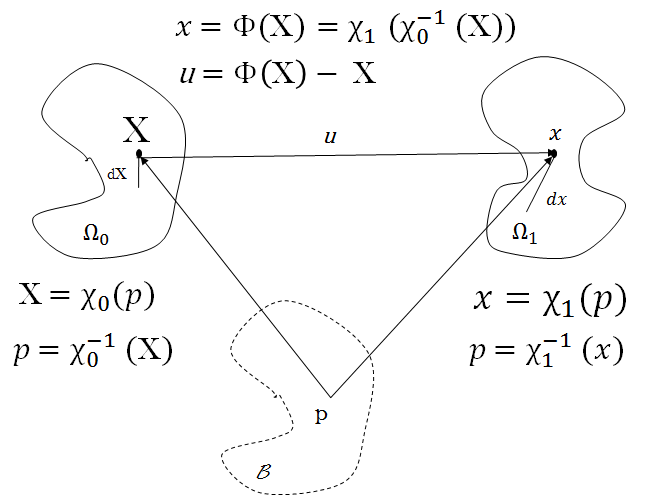
\includegraphics[width=0.7\textwidth,keepaspectratio]{figures/referenceFig.png} 
\caption[]{ }
\label{reference_config_theory}
\end{center}
\end{figure}

Suppose that $G(\Omega_1)$ is the value of some extensive physical property  associated with the body $\beta$ in the current configuration (such as the body mass $m$\nomenclature{$m$}{Body mass}). There exists a density $g(x)$ such that:
 $$G(\Omega_1) = \int_{\Omega_1} g(x)dv$$  
 where $dv$ is the volume of the material element.
 Thus, the property $G(\Omega_1)$ is related to the body while the density $g(x)$ is related to the position of the body particle.
\subsubsection*{Eulerian and Lagrangian formulations}
There are two classical techniques used to describe the body physical characteristics depending on the choice of independent variables.
 Some physical characteristics, such as mass density, can be defined for each individual particle. In such cases, the body characteristics are defined by the function $$m =  \mathcal{M}(p)$$ for all $p \in \mathcal{B}$. Here the coordinate system remains consistent and moves with the particle. Therefore, the coordinates of both, the particle and the attached variable, do not change along the deformation. A particle is an abstract entity and cannot be used in numerical calculations, thus it is described by its location in reference configuration $p= \chi_0^{-1}(X)$ .
 $$m =  \mathcal{M}(p) = \mathcal{M}(\chi_0^{-1}(X))$$
 We call $X$ Lagrangian or material coordinates and their application is called Lagrangian or material description.  
 

Instead of defining body characteristics as a function of body particles, one can define it directly as a function of particle location in current configuration by using the relation $ x = \chi_1(p)$, and therefore 
$$m = \tilde{ \mathcal{M}}(x) = \mathcal{M}(\chi_1^{-1}(x))$$
 Here the coordinate system is fixed and the particles coordinate are changing. Therefore, the position of particle and any related quantity changes during the deformation.We call $x$ Eulerian or spatial coordinates and their application is called Eulerian or spatial description.
 
 These approaches are distinguished by three important aspects: the mesh description, the stress tensor and momentum equilibrium and the strain measure. The advantages and drawback of these two formulations will be discussed later in this chapter. Further, only Lagrangian formulation is used to describe the continuous deformation of soft tissues.       

\subsubsection*{Deformation gradient}\label{deformatiogradient}

In mathematical formulation the deformation gradient tensor $F$\nomenclature{$F$}{Deformation gradient} is the Jacobian matrix of the deformation $\Phi(X)$:
\begin{equation}
F = \frac{\partial \Phi (X)}{\partial X} = \frac{\partial x}{\partial X}
\end{equation}

Considering infinitesimal quantities, the deformation gradient relates the segment $dX$ in the reference configuration to the corresponding deformed segment $dx$ in the current configuration (Figure \ref{reference_config_theory}) 
\begin{equation}
dx = F \cdot dX.
\label{deformationGradRelation}
\end{equation}

In addition to the mapping of such vectors, the deformation gradient tensor allows also the mapping of differential volumes as:
\begin{equation}
dv = det(F)dV = JdV
\end{equation}

The Jacobian determinant of the deformation gradient tensor $J$\nomenclature{$J$}{Jacobian determinant of the deformation gradient tensor} is a measure of the volume variation during the deformation. It can be used to relate extensive physical properties in the current and reference configurations:
\begin{equation}
\int_{\Omega_1}g(x)dv = \int_{\Omega_0}g(\Phi(X))JdV
\label{JacobianRelation}
\end{equation}

\subsubsection*{Decomposition of deformation gradient tensor into rotation and stretch}\label{deformationgradienttensor}
The deformation gradient tensor represents the entire body deformation, which consist of rigid body rotation and body "stretch" (see fig. \ref{deformationGradientDecom}). As $dX$ and $dx$ are differential segments, the map $F$ is not affected by rigid-body translations.
Generally, the body stretch is defined as the ratio of the deformed line elements to the length of the corresponding undeformed line element \nomenclature{$l$}{body stretch}:
\begin{equation}
l = \frac{\vert dx \vert}{\vert dX \vert}
\end{equation} 

Using polar decomposition theorem, the deformation tensor can be written as the product of a proper orthogonal tensor $R$ representing the rotational part, and a symmetric positive defined tensor $U$ representing the body distorsion. 
\begin{equation}
F = R \cdot U.
\end{equation}
where $U$ and $R$ are given by the relations $U = (F^T \cdot F)^ {\frac{1}{2}} $ and $R = F \cdot U^{-1}$. The tensor $U$ is also called the \textbf{right stretch tensor}.  Since there is a one-to-one relation between $U$ ans $U^2$, for the simplification of numerical calculus the stretch tensor can by replaced by the \textbf{Green deformation tensor} $C = F^T \cdot F$.


\begin{figure}
\begin{center}
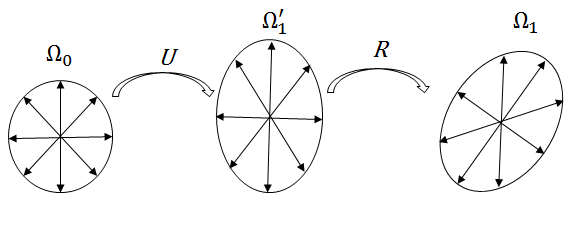
\includegraphics[width=0.7\textwidth,keepaspectratio]{figures/deformationTensorDecomposition.png} 
\caption[]{Decomposition by rotation and a stretch of a material particle.  }
\label{deformationGradientDecom}
\end{center}
\end{figure}

Where are three particular functions of $C$ called the principal scalar invariants.
\begin{equation}
\label{principal_invariants}
I_1(C) = tr C, \ \ I_2(C)=\frac{1}{2}\left[ trC^2 - \left(tr C \right)^2 \right], \ \ I_3(C)=det(C) 
\end{equation}
 The interpretation is that, the body "stretch" consists (locally) of three mutually orthogonal stretches, "the principal stretches".  The latter are scalar combinations of $C$ components that do not change under coordinate transformations for a given body configuration. The use of invariants will be an essential part of constitutive modeling, because the behavior of a material should not depend on the coordinate system.

It can be also shown that:

\begin{equation}
det(C-\mu I) = -\mu ^3+I_1(C)\mu ^2-I_2(C)\mu +I_3(C)
\end{equation}


\subsubsection*{Strain measures}\label{strainmeasure}
Referring to small deformations, the engineering nominal strain is defined as the ratio of the change in length of the deformed line element to the length of the corresponding undeformed line element:  
\begin{equation}
\epsilon = \frac{ dx  - dX }{	dX }
\end{equation}

Then the body is not deformed, the deformation gradient $F$ and therefore the right stretch tensor $U$ is equal to identity tensor $I$. The strain in such case is equal to zero. 

Then one is modeling biological soft tissues, large deformation have to be considered. Therefore, the previously defined strain is no more applicable. For large deformations, a measure of strain can be any monotonically increasing function related to stretch in a one-to-one manner and what completely vanishes in the reference configuration.

In orthogonal coordinate system, an admissible function is:
\begin{equation}
f(x) = \frac{1}{m}(x^m-1) \ \ (m \neq 0)\  \ and \ ln(x) \ \ (m=0)
\end{equation}   

Then $m=2$ the function is named the Green-Lagrangian stain tensor: 
\begin{equation}
E = \frac{1}{2}(U^2-I) =  \frac{1}{2}(C-I)
\end{equation}
The Green-Lagrangian tensor is commonly used in practice as it can be computed without prior knowledge of the eigenvectors of Green deformation tensor C.
%Here only Green-Lagrangian strain is introduced. The Green-Lagrangian tensor $E$ is defined as:
%\begin{equation}
%dx^2 - dX^2 = 2dX \cdot E \cdot dX
%\label{GLRelation}
%\end{equation}
%
%From \ref{deformationGradRelation} equation, $dx^2$ is written as
%$$dx \cdot dx = (F \cdot dX)\cdot (F \cdot dX) = (F \cdot dX)^T \cdot (F \cdot dX) = dX^T \cdot F^T \cdot F \cdot dX = dX \cdot C \cdot dX,$$
%therefore the relation \ref{GLRelation} becomes 
%$$dX \cdot C \cdot dX - dX \cdot I \cdot dX = dX\cdot 2E \cdot dX$$
%Since the above relation must hold for all $dX$, one can deduce that:
%\begin{equation}
%E = \frac{1}{2} (C - I)
%\end{equation}

\subsection{Stress measures}%\label{subsection:stressmeasure}

\subsubsection*{Body and contact forces}\label{bodycontactforces}
Generally, forces are categorized as internal and external forces. An \textbf{external force } is a force caused by an external agent outside of the system, and contrariwise an \textbf{internal force} is a force exchanged by the particle in the system. The external forces, in turn, are categorized in \textbf{body forces} (acting at the distance) and \textbf{contact forces} (acting on the body surface). The relation between body forces per unit undeformed volume $\tilde{b}(X)$ (Lagrangian coordinates) and body forces per unit deformed volume $b(x)$ is given by the following relation:
\begin{equation}
\tilde{b} = \frac{dv}{dV} b = Jb.
\end{equation}

The contact forces can act on the external surface of the body or on a imaginary internal surface enclosing a volume element (Fig. \ref{internalcontactForceDefinition}). 
In general terms, the stress (or the \textbf{traction vector}) $t^n(x)$ is defined as contact force per unit area $da$ in the limit as $da \rightarrow 0$. Therefore $t^n(x)$ varies from point to point in intensity and orientation depending on the $da(n)$ orientation.  The stress vector projection on normal axis $n$ define the \textbf{normal stress vector} and it's projection on the tangential axis define the \textbf{shear stress vector}.


\begin{figure}
\begin{center}
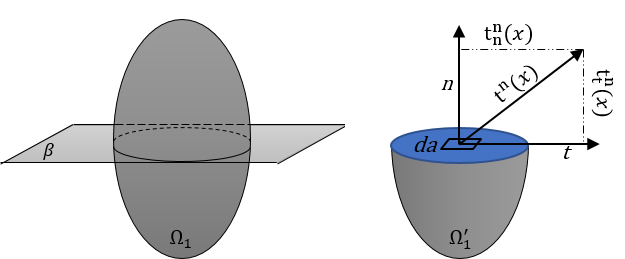
\includegraphics[width=0.7\textwidth,keepaspectratio]{figures/internalcontactForceDefinition.png} 
\caption[]{True stress vector $t^n(x)$ at point $x$ on the fictitious surface created  by the cutting plane $\beta$ of normal  $\overrightarrow n$ passing through the point $x$. }
\label{internalcontactForceDefinition}
\end{center}
\end{figure}

The stress on the boundary $\partial \Omega_1$ of the region occupied by the studied body is applied by external forces through physical contact along the boundary. When formulating and solving a boundary-value problem, this stress define the boundary conditions.




\subsubsection*{Cauchy's lemma}

Cauchy's lemma states that traction vectors acting on opposite sides of a surface are equal and opposite.
\begin{equation}
t^{-n}(x) = -t^n(x)
\label{chauchyLemma}
\end{equation}
\subsubsection*{Cauchy's Law}
Cauchy’s law states that there exists a Cauchy stress tensor $\sigma$ which maps linearly the normal to a surface to the stress vector acting on that surface, according to the next relation
\begin{equation}
t^n = \sigma \cdot n \ \ \ where \  \ t^n_i = \sigma_{i,j} n_j
\end{equation}

Then large deformations are considered, the reference and current configurations of the body are significantly different and a clear distinction has to be made between them. The traction vector $t^n$ is defined in Eulerian coordinates (body current configuration) and is also called the \textbf{true stress}. Accordingly, the Cauchy stress tensor $\sigma$ is called the true stress tensor.

The definition of any measure with respect to the deformed configuration is less practical as the current configuration is usually unknown a priori. For the simplification of mathematical formulation, a new pseudostress is defined in the Lagrangian coordinate space named \textbf{engineering stress}. The engineering stress have no physical meaning and have to be converted in to true stress for any interpretations.


\begin{figure}
\begin{center}

\includegraphics[width=0.7\textwidth,keepaspectratio]{figures/stressnotion.png} 
\caption[]{Deformation of area $dA$  into area $da$. The force $df$ acting on deformed area $da$ and the pseudoforce $d\tilde{f}$ acting on undeformed area $dA$}
\label{stressnotion}
\end{center}
\end{figure} 


Next, two pseodostress vectors are defined (Fig. \ref{stressnotion}):
\begin{itemize}
\item the contact force $df$ per unit area in reference configuration  $dA$.
\item the contact pseudoforce $d\tilde{f}$ per unit area in reference configuration $dA$.  
\end{itemize}

Accordingly, two pseudostress tensors are defined based on pseudostress vectors:
\begin{itemize}
\item $T^N = P \cdot N$, $P$ is called \textbf{first Piola-Kircchoff stress tensor},
\item  $\tilde{T}^N = S \cdot N $, $S$ is called \textbf{second Piola-Kircchoff stress tensor}. 
\end{itemize} 
The three stress tensors are linked by the next relation 
\begin{equation}
\sigma = J^{-1}F \cdot P = J^{-1} F \cdot S \cdot F^T
\label{PK12}
\end{equation}
\readysubsection{Conservation equations}%\label{subsection:conservationequations}
Three conservation low must to be satisfied by physical system subject to any applied boundary conditions: \textbf{conservation of mass, conservation of linear momentum} and \textbf{conservation of angular momentum}. The resulting equations describe partially the mechanical behavior of a continuous body.

\subsubsection*{ Conservation of mass}
The mass $m$ of a body with the density $\rho$, that infill the space region $\Omega_1$ is given by :
\begin{equation}
m(\Omega) = \int_{\Omega} \rho(X)dV
\end{equation}
The mass conservation low requires that the body mass remain constant throughout all possible body configurations. For a Lagrangian formulation, this results in a relation between the body density in the reference configuration $\rho_1$ and the body density in the current configuration $\rho$.
$$\int_{\Omega_1} \rho_1 dv = \int_{\Omega_0} \rho_0 dV = const. $$

Using the relation \ref{JacobianRelation} one can deduce that:
\begin{equation}
\int_{\Omega_0} \left( \rho_1 J - \rho_0\right)dv = 0 \  \ and \  \ \rho_1 J = \rho_0
\end{equation}
\subsubsection*{Conservation of the linear momentum}
Assume that a body $\beta$ defined on a arbitrary region $\Omega_1$ with boundary $\Gamma_1$ is subjected to a body-force $\rho  b$ and the surface traction $a t^n$. And let $X$ be the particle location in the deformed solid.
 The total force acting on the body $\beta$ is defined as:
\begin{equation}
f = \int_{\Omega_0}\rho_0 b(X)dV + \int_{\Gamma_0} T^N(X)dA
\end{equation}
 
The conservation of the linear momentum requires that the total forces acting on the body to be equal to the time rate change of the linear momentum. In a static problem the time rate change of the linear momentum is neglected and thus the next equilibrium equation is obtained.
\begin{equation}
\rho_0 b+\nabla_0 \cdot P  = 0
\end{equation}
here the $P_{ji}$ are the components of first Piola-Kircchoff stress tensor
The equilibrium equation can be formulated in therms of the second Piola-Kircchoff stress tensor by using \ref{PK12} relations.
\subsubsection*{Conservation of angular momentum}
The conservation of angular momentum requires that the resultant momentum on any part of the body about a fixed point $\mathcal{O}$ equals the rate of increasing of its angular momentum (about $\mathcal{O}$). For a static problem, the integral form of the conservation of angular momentum is defined as:
\begin{equation}
\label{angularMomentum}
\int_{\Omega_0} X \times \rho_0 b(X)dV + \int_{\partial \Omega_0} X \times  T^N(X)dA = 0
\end{equation}

The relation \ref{angularMomentum} demands that the second Piola-Kircchoff stress tensor by a symmetric tensor:
\begin{equation}
S = S^T
\end{equation}
In summary, the conservation equations are fulfilled if and only if the following local conditions are fulfilled at each point in the body:
\begin{equation}
\rho_1 J = \rho_0, \ \ \nabla_0 \cdot S \cdot F^T + \rho_0 b =0, \ \ S=S^T 
\end{equation}
with the traction on the surface related to the stress through $\tilde{T^n} = S \cdot N$.
 For the simplification of mathematical calculus, the constitutive equations are formulated in therms of the second Piola-Kircchof stress tensor using the relations \ref{PK12}.

\subsubsection*{Govering equations of Lagrangian formulation} 
We consider a body $\beta$ which occupies in the reference configuration the domain $\Omega_0$ with a boundary $\Gamma_0$`. The governing equations for the mechanical behavior of a continuous body are:
\begin{enumerate}
\item Conservation of mass $\rho_1 J = \rho_0$
\item Conservation of linear momentum $\nabla \cdot P + \rho b = 0$
\item Conservation of angular momentum $F \cdot P = P^T \cdot F^T$
\item Constitutive equations
\item Measure of strain $E = \frac{1}{2} (C-I)$
\item Boundary condition: $e_i \cdot N \cdot P = e_i \cdot \overline{t}$ on $\Gamma_0^{t_i}$
\item Internal continuity condition: $\llbracket e_i \cdot N \cdot P \rrbracket = 0$ on $\Gamma_0^{int}$
\end{enumerate} 

Where we note $\Gamma_0^{t_i}$ the set of prescribed traction  $\overline{t}$ on the body boundary $\Gamma_0$ ; and $\Gamma_0^{int}$ is the union of all surfaces where the stresses are discontinuous in the body (material interfaces).

The momentum equation together with the traction boundary condition and interior traction continuity condition are called Generalized Momentum Balance (GBM).


\readysubsection{Constitutive models}%\label{subsection:constitutivemodels}
   The constitutive models, called also material models, define the relation between stress and strain of a physical system under the action of a external stimuli. It is very complex to define a universal material behavior capable to model the material response to all possible conditions. Thus, for one martial, several constitutive models can be defined depending on the studied characteristics. \\
	Based on different characteristics biological materials are classified into:
	\begin{itemize}
\item \textit{ Isotropic or anisotropic materials:} the response of a isotropic (anisotropic) material to an applied load is independent (dependent) of the direction of loading.
\item\textit{ Compressible or incompressible materials:} in a compressible (incompressible) material the volume is changed (unchanged) during the deformation and the density remains constant. For a incompressible material the Jacobian determinant of the deformation tensor $J$ is equal to 1. 
\item \textit{ Homogeneous or heterogeneous materials} the response of a homogeneous (heterogeneous) materials is independent (dependent) of the position within the body.
	\end{itemize}

Biological soft tissues are modeled using elastic materials model. The elasticity is the property of a solid material to return to its original size and shape when the influence of a external force is removed. In this case the strains are said to be reversible. 
	 
Considering small deformations, the stress-strain law of a linear material is given by the \textbf{Hook's law} $$\sigma = \lambda \epsilon,$$ where  the coefficient of proportionality $\lambda$ is named \textbf{Young's modulus}. \\
For large deformation the stress-strain relationship is deduced from a potential function. A \textbf{hyperelastic} material is an elastic material for which the work is independent of the deformation path. The material reversibility and path-independent behavior implies the absence of energy dissipation during the deformation. Thus there exist a \textbf{potential} function $W(\epsilon)$ such that $$S = \frac{\partial W(E)}{\partial E}= 2\frac{\partial \psi (C)}{\partial C}$$.\\
Moreover, if the material is isotropic, the stored strain energy $W$ of a hyperelastic material can by written as a function of principal invariants ($I_1, I_2, I_3$) of the Green deformation tensor $C$ previously defined in equation \ref{principal_invariants}. Next, we introduce the most used potential functions for characterization of biological soft materials.
 
For the simplification of potential expressions we define the first and the second deviatoric strain invariant :
\begin{center}
$\overline{I}_1=\frac{I_1}{I_3^{1/3}} $;  $\overline{I}_2=\frac{I_2}{I_3^{2/3}}$
\end{center}

We also define the \textit{ bulk modulus} as measure of a material's resistance to compression; the shear modulus as the ration of shear stress to the shear strain; and the Poisson ratio as the ration between longitudinal strain to the transverse strain describing the body shape change . For small deformation the bulk modulus and shear modulus are linked to the Young's modulus and Poisson ration by the next relations:
 \begin{center}
  $K = \frac{E}{3(1-2\nu)}$ and $\mu = \frac{E}{2(1+\nu)}$
 \end{center}
  
\subsubsection*{Neo-Hookean potential function}
The Neo-Hooken low is an extension of the Hook's low to large deformations. The potential function is based only on the first invariant and is given by 
\begin{equation}
\label{Neo-Hook}
W =\frac{\mu}{2} (\overline{I}_1-3) + \frac{K}{2}(J-1)^2
\end{equation}
Where $\mu$ and $K$ are initial shear modulus and initial bulk modulus respectively. 
\subsubsection*{Mooney-Rivling potential function}
The potential function of a Mooney-Rivling material is defined as:
\begin{equation}
W=\frac{\mu_1}{2}(\overline{I}_1-3)+\frac{\mu_2}{2}(\overline{I}_2-3)+\frac{K}{2}(J-2)^2
\end{equation}
Where the constants $\mu_1$ and $\mu_2$ describing the material properties are linked to the initial shear modulus $\mu = (\mu_1+\mu_2)$. And the constant $K$ is the initial bulk modulus. 
\subsubsection*{Gent potential function}
The potential function of a Gent material model is defined as:
\begin{equation}
W=-\frac{\mu J_m}{2}ln\left(1-\frac{\overline{I}_1-3}{J_m}\right)+\frac{K}{2}\left(\frac{J^2-1}{2}-lnJ\right)
\end{equation}
 Where, as previous the $\mu$ and $K$ constants are the initial shear modulus and the initial bulk modulus respectively. And $J_m$ is the limiting value of $(\overline{I}_1-3)$

\readysection{Finite Element Discretization}

\label{section:lagrangianmesh}
As previously described, in continuous mechanics the body deformation is expressed in terms of partial differential equations (PDE). For the majority of problems, the PDEs cannot be solved analytically, therefore approximation methods are developed. To this end, the finite element (FE) method has become the standard numerical calculation to compute such approximations. The computational domain, the unknown solution, and its partial derivatives are discretized, so as to obtain a set of algebraic equations for the function values at a finite number of discrete locations. The unknowns of the discrete problem are
associated with a computational mesh which represents a subdivision of the domain $\Omega_0$ into many small control volumes $\Omega_k$

\readysubsection{Eulerian and Lagrangian mesh description}

The mesh description depends on the chosen independent variables (Eulerian or Lagrangian formulation). In a Eulerian mesh, the Eulerian coordinates of nodes are fixed (coincident with spatial points) and the material point change in time (see Figure \ref{lagrangian_mesh}.b). In this case the mesh has to be large enough to contain the body in its current configuration. Throughout the deformation the material points will belong to different elements. Whereas, in a Lagrangian mesh, the Lagrangian coordinates of nodes are time invariant, nodal trajectory corresponds with material points trajectory and no material passes between elements (see Figure \ref{lagrangian_mesh}.a). 

\begin{figure}[!h]
\centering
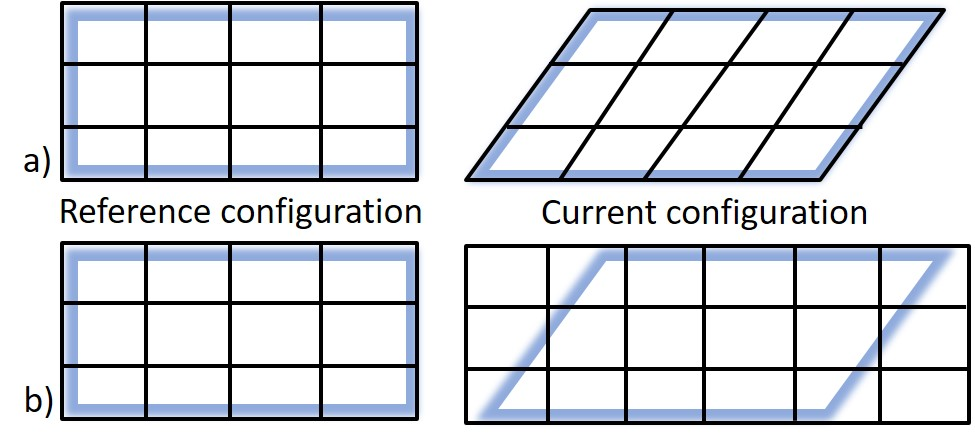
\includegraphics[width=0.8\textwidth,keepaspectratio]{figures/lagrangian_mesh.jpg} 
\caption{a) Lagrangian mesh formulation. b) Euler mesh formulation}
\label{lagrangian_mesh}
\end{figure}
 

In a Lagrangian mesh the boundary and interface nodes remains coincident with body boundaries and material interfaces throughout the entire deformation. Thus, the boundary conditions are defined directly on the respective nodes. On the other hand, in a Eulerian mesh the boundary and interface conditions have to be defined on point which are not nodes. This implies important complications in multi-dimensional problems.  

An important drawback of a Lagrangian mesh affect mainly the large deformation domain. As the nodes are coincident with the material points, the elements deform with materials. Therefore, the magnitude of deformation is limited because of element distortion. The limited distortion that most elements can sustain without performance degradation or failure is a important factor in nonlinear analysis with Lagrangian formulation. 

In conclusion, an Eulerian mesh formulation is usually used to solve problems linked to fluid like materials and a Lagrangian mesh for solid like materials.

\readysubsection{Lagrangian mesh}\label{subsection:lagrangianmesh}

The general approach of the FE method in Lagrangian formulation is shown in Fig. \ref{fe_method}. First the momentum equations with given boundary conditions is multiplied by an appropriate test functions. The test function has to satisfy all displacement boundary conditions and to be smooth enough so that all derivatives in momentum equations are well defined. Then performing an integration by parts, the week formulation of GBM is obtained, also called the principle of virtual work. \textcolor{darkred}{cite Belytschko}

\begin{figure}[!h]
\centering
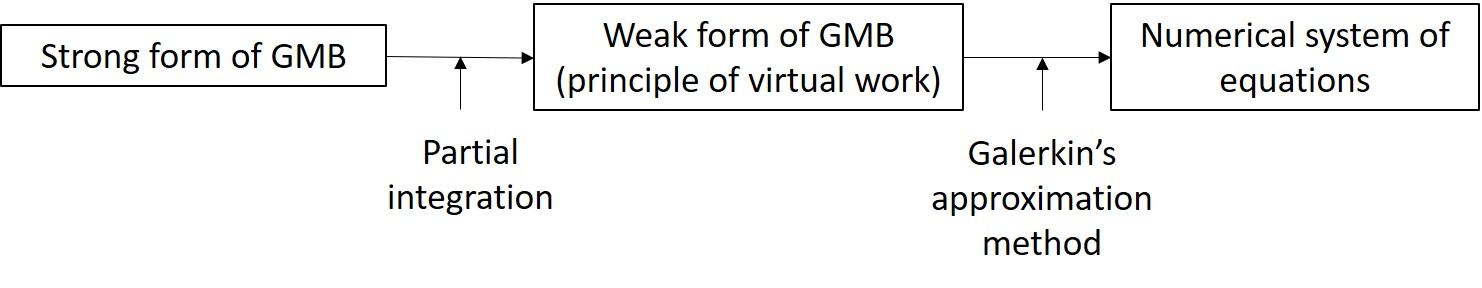
\includegraphics[width=0.8\textwidth,keepaspectratio]{figures/fe_method.jpg}
\caption{From strong formulation of the generalized momentum balance to numerical equations.}
\label{fe_method}
\end{figure}




 The momentum equations and the traction boundary conditions, usually called the strong form, cannot be directly discretized by FE method. The strong formulation of the GBN equations impose the $C_1$ continuity conditions on the field variables. Therefore, the solution of this problem does not always exist. This is true especially in the case of complex domains with different material interfaces. In order to overcome these difficulties, weak formulations are preferred. The week formulation of GMB reduce the continuity requirements thereby allowing the use of easy-to-construct and implement polynomials. Because of the reduction in the requirements of function smoothness, the weak forms never give an exact solution but one can obtain a relatively accurate solution with the discretization refinement.



From the week form of the GBM equations, the numerical system of equations is formulated by using finite elements interpolants for the mechanical displacement and the test functions.   The whole domain is discretization into a number of smaller areas or volumes which are called \textbf{finite elements} and their assembly is called a\textbf{ mesh}. Elements can be of various shapes (as shown in Figure \ref{discretization}.a),  quadrilateral or triangular in two dimensions, and tetrahedral or hexahedron in three-dimensions.


\begin{figure}[!h]
\centering
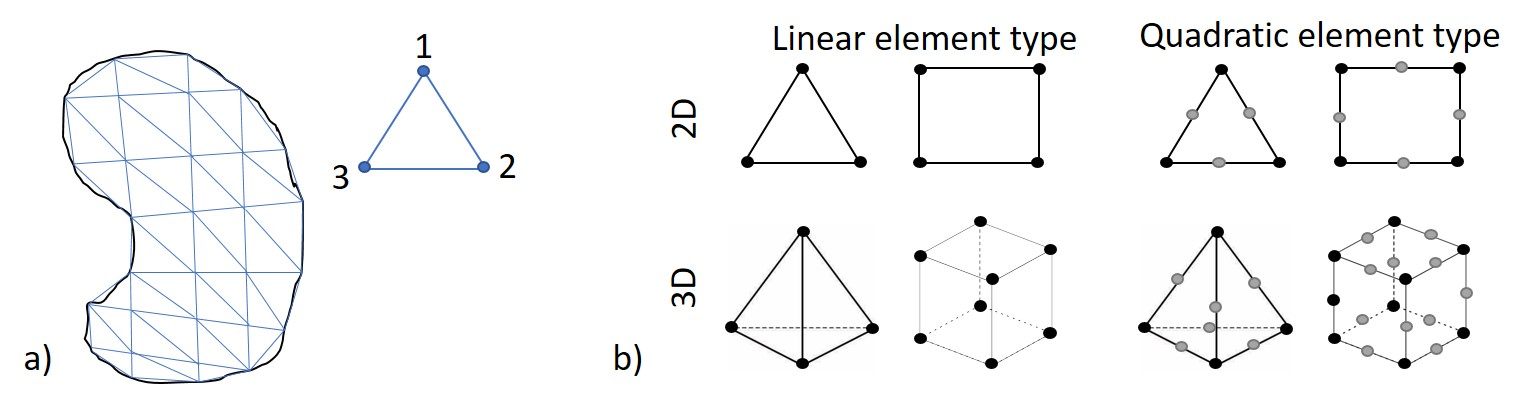
\includegraphics[width=1\textwidth,keepaspectratio]{figures/discretization.jpg} 
\caption{a) Discretization of  a 2D domain with triangular finite elements :Lagrangian mesh . b) Different types of finite elements}
\label{discretization}
\end{figure}

 The mechanical displacement is approximated at the discretization points called finite element\textbf{ nodes}. The nodes are at the corners of the elements for a linear type, and at the corners and midsides of the elements for a quadratic type (figure \ref{discretization}.b). The displacement of each point within an element is fixed by the values of the displacements of the nodes of the element. In this way, the problem of finding the displacement of every point within the body is replaced by the problem of finding the displacements of a finite number of points.
 
 As in a Lagrangian mesh the nodes are following the motions, for large deformation the finite elements can be highly distorted. Therefore, the shape quality is generally followed all along the deformation process. Several shape parameters as a function elements geometry have been proposed as: aspect ratio, maximum corner angle, Jacobian ratio, skewness, parallel deviation, warping factor. The acceptable limit values are proper to the elements types. 
 
In the following only shape parameters of linear triangular elements are presented.  
 \subsubsection*{Triangle aspect ratio }
 The element's shape aspect ratio is computed using only the corner nodes of the element (Figure \ref{fig:aspectratio}). First, two lines are created: one through a node ($K$) and the midpoint of the opposite edge ($ K'$), the second through the midpoint of the others two edges ($J'$ and $ I'$). Then two rectangles are created, each rectangle have a pair of edges parallel to one of previously defined lines. The rectangle edges have to pass through the nodes and the triangle's edges midpoints. This construction is repeated for each triangle's node resulting in 6 rectangles. The aspect ratio of a rectangle is defined as the ration between the longer and shorter side. Thus, the triangle's aspect ratio is defined as the maximal aspect ratio over the 6 rectangles divided by squared root of 3. 
 
 The best possible aspect ratio is 1 and is represented by an equilateral triangle. An element with an aspect ratio larger than 20 is considered as bad aspect element, large aspect ratio may degrade solution performance.
 
 \begin{figure}[!h]
\centering
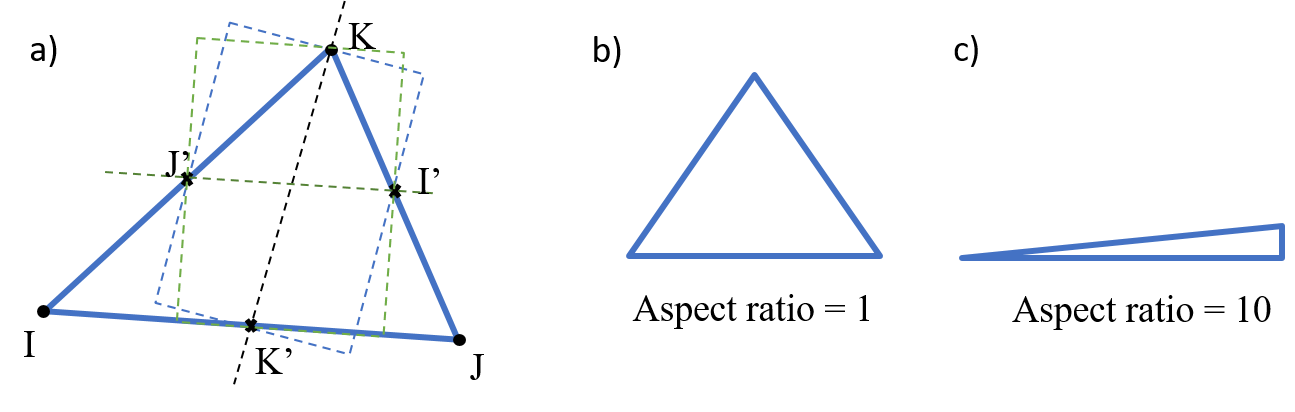
\includegraphics[width=0.9\textwidth,keepaspectratio]{figures/aspectRatio.png} 
\caption{Computation of aspect ratio for a triangle}
\label{fig:aspectratio}
\end{figure}  

\subsubsection*{Triangle maximum corner angle}
The maximum corner angle is computed using nodes position in 3D space. The best possible maximum corner angle is 60\textdegree. An element having a maximal corner angle larger than 165\textdegree is considered as bad shape element, large corner angles may degrade the solution performance. Figure \ref{fig:cornerangle} shows a triangle with a good ( 60\textdegree) and bad ( 165\textdegree) quality. 

 \begin{figure}[!h]
\centering
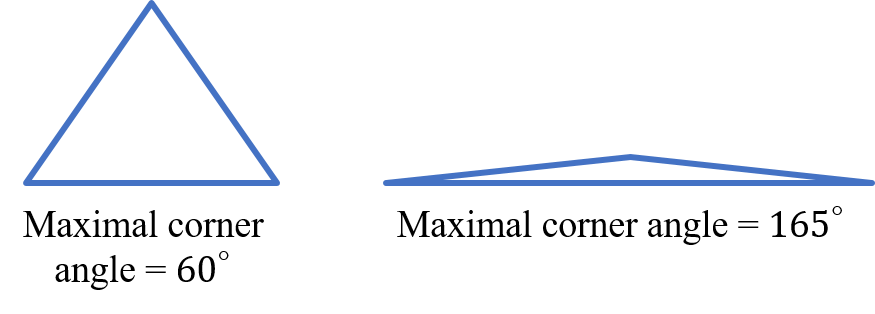
\includegraphics[width=0.6\textwidth,keepaspectratio]{figures/maximalcornerangle.png} 
\caption{Example of triangles with different maximal corner angles.}
\label{fig:cornerangle}
\end{figure} 

The aspect ratio and the maximal corner deviation of a tetrahedra is computed using the definition of the same measure on a triangle. The elements shape parameter is assigned as the worst value over the triangles defined by the tetrahedra's faces and cross-sections.  

\subsubsection*{Skewness }
The skewness of a triangular element is computed using the equivalent volume deviation method. It is defined as the difference between the optimal and real cell size over the optimal cell size. The optimal size is the size of an equilateral cell with the same circumradius. According to its definition, the value of 0 indicates an ideal cell, from 0 to 0.75 the cell is considered to have a good quality, from 0.75 to 1 the cell is considered to have a bad quality and a value of 1 indicates a completely degenerated cell (Figure \ref{fig:skewness}).   

 \begin{figure}[!h]
\centering
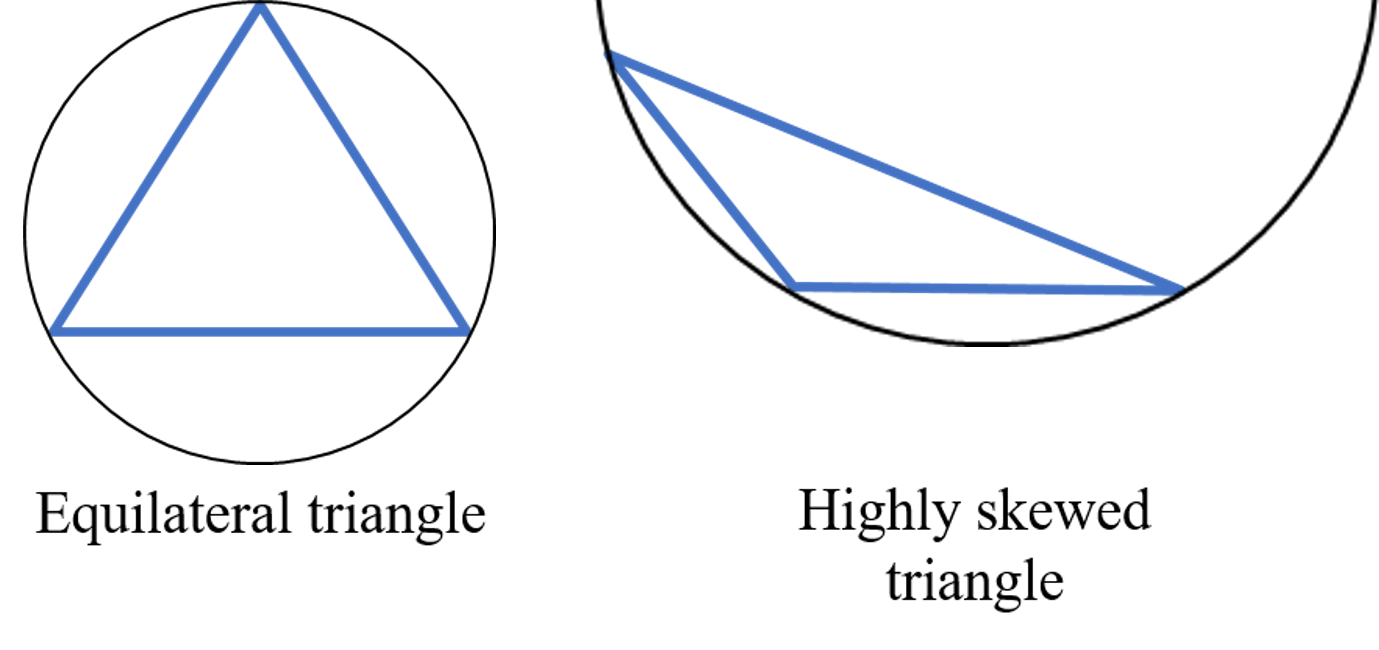
\includegraphics[width=0.6\textwidth,keepaspectratio]{figures/skewness.png} 
\caption{Example of triangles with different skewness.}
\label{fig:skewness}
\end{figure}
 
\readysection{Contact mechanics}\label{section:contactmechanics}

In order to transfer the loads between elements, the nodes have to be connected together. If two bodies are separated with no commune nodes, no interaction will occur during the deformation and the bodies will pass through each other. Here, an asymmetric surface-to-surface contact method is used to solve the multi-body interaction problems.

Let's consider two different bodies $\mathcal{A}$ and $\mathcal{B}$ and their occupied domains $\Omega_A$ and $\Omega_B$ with boundaries $\Gamma_A$ and $\Gamma_B$ respectively (see Figure \ref{contact_bodies}). Also, we note $\Omega$ the domain of intersection of two bodies. The contact interface is the intersection of the surfaces of the two bodies:
$$\Gamma = \Gamma_A \cap \Gamma_B.$$
The intersection consists of two surfaces distinguished as \textbf{target} and \textbf{contact} surfaces. The choice of the surfaces is made following the next guidelines:
\begin{itemize}
\item if the one body $\mathcal{A}$ is stiffer then the body $\mathcal{B}$, the surfaces $\Gamma_A$ define the target and $\Gamma_B$ the contact surface;
\item if $\Gamma_A$ is a concave surface getting in contact with the convex surface $\Gamma_B$, the surface $\Gamma_A$ define the target and $\Gamma_B$ the contact surface.
\item if the surface $\Gamma_A$ is larger than $\Gamma_B$, the surface $\Gamma_A$ denote the target and the $\Gamma_B$ the contact surfaces.
\end{itemize} 
For the following, we identify $\Gamma_A$ as the target surface and $\Gamma_B$ as the contact surface (Figure \ref{contact_bodies}).
\readysubsection{Contact inteface equations}%\label{governingequations}
 In multi-body interaction process, in addition to standard governing equations, two more contact conditions have to be fulfilled: the two bodies cannot interpenetrate and the traction must satisfy momentum conservation on the contact interfaces.
   

 \begin{center}
\begin{figure}
\centerline{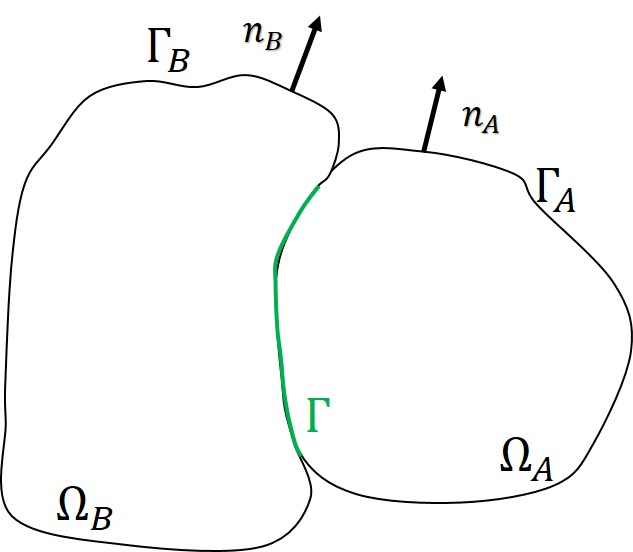
\includegraphics[width=0.4\textwidth,keepaspectratio]{figures/contact_bodies.jpg} }
\caption{Multi-body contact problem.}
\label{contact_bodies}
\end{figure}
\end{center} 
   
  \subsubsection*{Traction conditions}
  Traction conditions must follow the balance of momentum across the contact interface:
  \begin{equation}
  t_A + t_B=0
\end{equation}
On the contact boundary surface $\Gamma$ the traction vectors is decomposed into it's normal and tangential components:

$$t_A^n = t_A \cdot n_A,  \ \ \ t_B^n = t_B \cdot n_B$$
$$t_A^t = t_A - t_A^n n_A, \ \ \ t_B^t = t_B - t_B^n n_B$$

Therefore the momentum balance requires:
\begin{equation} 
t_A^n + t_B^n = 0, \ \ \ t_A^t + t_B^t = 0
\end{equation} 

 \subsubsection*{Inter-penetrability condition}
The bodies implied in a multi-body problem must fulfill the inter-penetrability condition:
\begin{equation}
\Omega_A \cup \Omega_B = 0
\end{equation}
Decomposing the displacement $u$ into normal and tangential components $u^n$ and $u^t$ respectively the inter-penetrability condition can be written as:
\begin{equation}
t^n \leq 0, \ \ u_n-g \leq 0, \ \ t_n(u^n-g) = 0
\end{equation}
 Where $g$ is the gap between the two bodies.

\readysubsection{Surface interaction models}%

\label{subsection:surfaceinteractionmodels}
When two solid bodies are placed together under a nonzero normal force and acted upon by another tangential force, a \textbf{friction force} $f_{friction}$ tangential to the interface and opposite to the applied force is created. Depending on whether the applied force can overcome the friction force opposing it, the bodies may or may not move relative to the other. The body motion along the interface is called \textbf{sliding}. The \textbf{sliding force}, $f_{sliding}$ is the applied tangential force which cause the sliding motion between the two bodies.
  
The problem in determining whether relative motion will or will not occur is one of balancing the involved forces. According to allowed relative body motion in tangential or normal directions, five types of surface interaction models are distinguished: bonded, rough, no-separation, frictional and frictionless. Table \ref{contactB} resume each mechanical behavior. If the body motion is not allowed in normal or tangential direction, once the bodies get in contact, the respective components of traction are equals $t_A=t_B$ . Which means that, for a pure \textbf{bonded} contact, the two bodies are considered as a unique solid body.    

\begin{table}[H]

\begin{center}
\begin{tabular}{||c|c|c||}
\hline
Name & body motion in normal direction & body motion in tangential direction \\
\hline\hline
Bonded & No & No\\
\hline
Rough & Yes & No, $f_{friction} \gg f_{sliding}$ \\
\hline
No-separation & No & Yes,  $f_{friction} = 0$ \\
\hline
Frictionless & Yes & Yes, $f_{friction} = 0$ \\
\hline
Frictional & Yes & Yes, if $f_{sliding} > f_{friction}$\\
\hline
\end{tabular}
\caption{Surface interaction models and behaviors}
\label{contactB}
\end{center}
\end{table}

\textit{Frictional} contact behavior is defined using Coulomb friction low.
For a continuous body the Coulomb friction model is applied at each point of the contact interface.
Consider that bodies $\mathcal{A}$ and $\mathcal{B}$ which are in contact within the surface $\Gamma$, then for all $x \in \Gamma$ :
\begin{equation}
\label{stiking}
if \ \Vert t^t(x) \Vert < -\mu_f t^n(x),\ \ \Delta u^t=0 
\end{equation}
\begin{equation}
\label{sliding}
if \ \Vert t^t(x) \Vert = -\mu_f t^n(x),\ \ \Delta u^t=-k(x)t^t(x),\ \ k(x)>0
\end{equation}

Where $\mu_f$ is the material property named \textbf{friction coefficient},  $\Delta u^t$ is the slip incremental in the tangential direction and $k(x)$ is a variable computed from the momentum equation. The condition \ref{stiking} is known as sticking condition: the tangential traction is less than the critical value, thus no sliding occurs. Reciprocally, condition \ref{sliding} is called sliding condition.

Then a frictionless contact model is used, $\mu_f = 0$, the tangential tractions vanish completely: $t_A^t = t_B^t = 0$. Then rough contact is modeled the friction coefficient $\mu_f$ is equal to infinity, therefore sticking condition is always fulfilled. 

Several contact models can be combined to model a physical contact between two bodies.   

\readysubsection{Contact formulation algorithm: Pure Penalty model}%\label{subsection:purepenalty}

\subsubsection*{Pinball region}

Contact problem present two primary difficulties. First is the traction conditions computation when frictional models are considered. And second is the unpredictability of regions which will get in contact with each other during the deformation process.

The region of contact depends on materials properties and imposed boundary conditions; therefore, it is very difficult to know a priori where the surfaces will come in contact. To formulate analytic equations, one has to know exactly the nodes involved in the contact process. Therefore, during the body deformation the program calculates if the contact is opened or closed. The status is defined using a sliding pinball (Figure \ref{pinball}). The pinball slide over the contact surface points and search for the target surface. If the node to surface distance is smaller than the pinball radius the contact is considered closed otherwise the contact is considered opened.   

 \begin{center}
\begin{figure}
\centerline{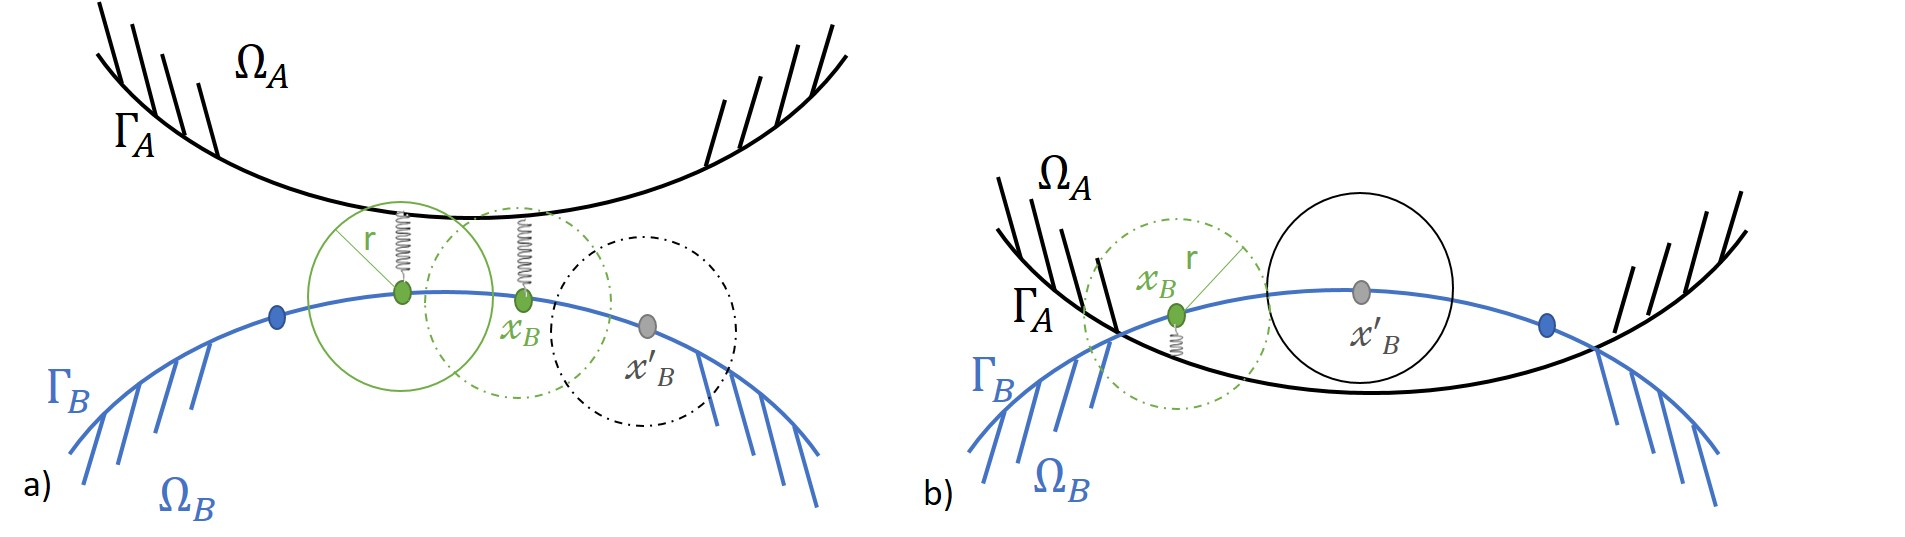
\includegraphics[width=1\textwidth,keepaspectratio]{figures/pinball.jpg} }
\caption{Contact status update using a pinball of radius r.}
\label{pinball}
\end{figure}
\end{center}
 
 \subsubsection*{Distance measures} 
  Let's consider a point $x_B$ bellowing to the body surface $\Gamma_B$ and $x_A$ the intersection point of the surface normal $n_B$ with the surface $\Gamma_A$ (Figure \ref{gap_penetration}). The point to surface distance $d_1(x_B,\mathcal{A})$  is defined as:
\begin{equation}
\label{normalContactdistance}
d_1(x_B,\mathcal{A}) = \Vert x_B-x_A \Vert = \left[  \Sigma_{i={1,2,3}}\left( x_B^i - x_A^i \right)^2\right]^{\frac{1}{2}}
\end{equation}

 \begin{center}
\begin{figure}
\centerline{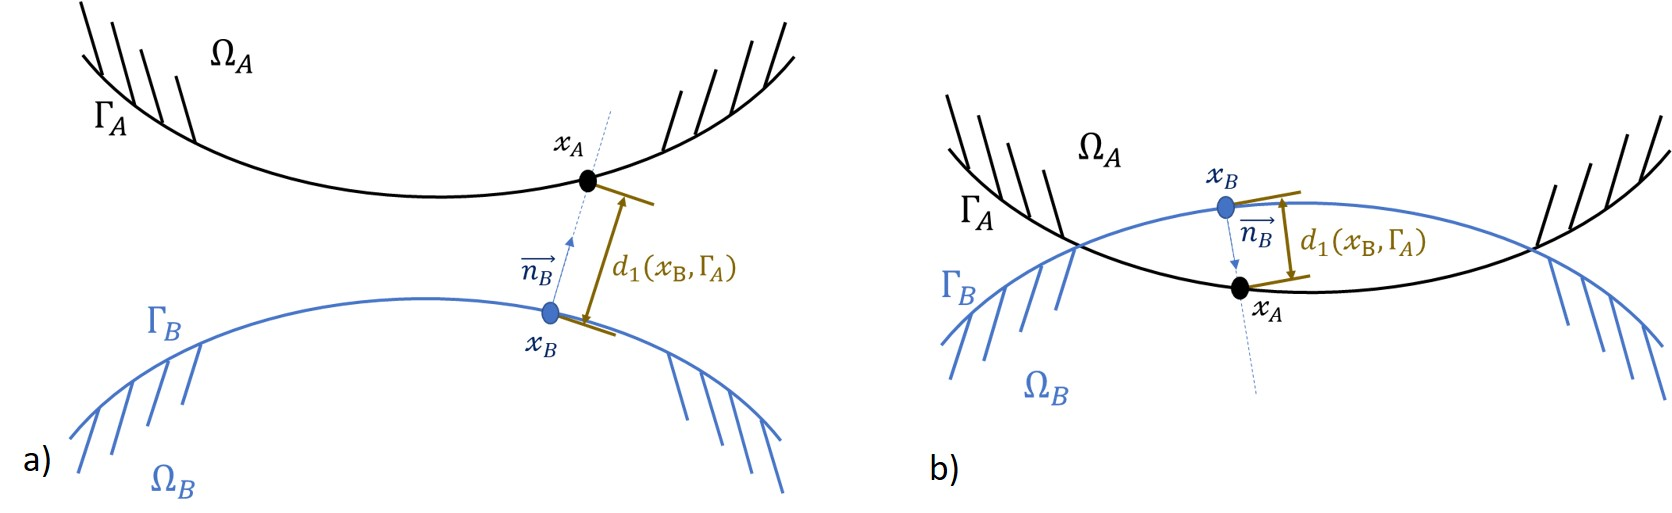
\includegraphics[width=1\textwidth,keepaspectratio]{figures/gap_penetration.jpg} }
\caption{  a) Body $\mathcal{A}$ and body $\mathcal{B}$  are close but not in contact. The  $d_1(x_B,\mathcal{A})$ measure define the gap between the bodies at point $x_B$.  b) Body $\mathcal{B}$ have penetrated the body $\mathcal{A}$. The $d_1(x_B,\mathcal{A})$ measure gives the penetration at point $x_B$.}
\label{gap_penetration}
\end{figure}
\end{center}

If the intersection point $x_A$ is located inside the pinball area, the node to surface distance define the amount of \textbf{gap} or \textbf{penetration} at the respective point (Figure \ref{gap_penetration}).
 
Computing the gap or penetration at single points increase numerical instabilities.  Therefore, in this work, the gap and penetration are computed in an averaged manner over the projected surface areas. Figure \ref{projecte_surface} show the projected surface areas (c) obtained by the intersection of the target surface (a) with the projected contact surface (b). 

 \begin{center}
\begin{figure}
\centerline{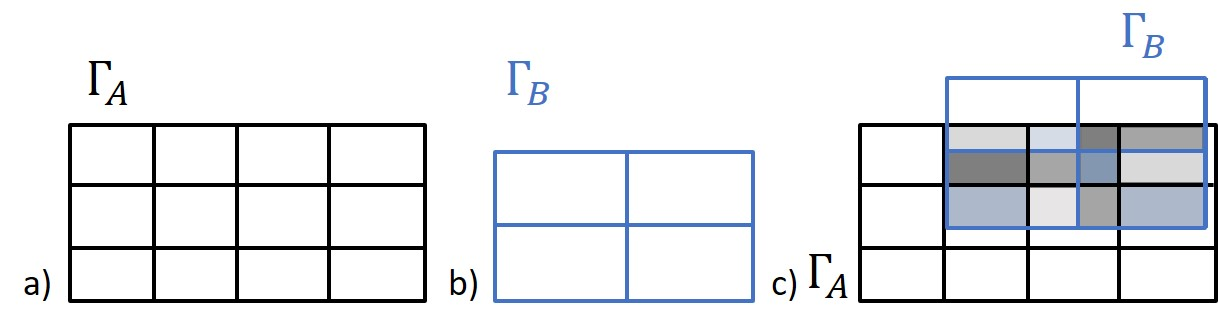
\includegraphics[width=1\textwidth,keepaspectratio]{figures/projecte_surface.jpg} }
\caption{The contact surface projection over the target surface: a) Target discretized area; b) contact discretized area; c) intersection of the projected surfaces.}
\label{projecte_surface}
\end{figure}
\end{center}

 The interested reader is referred to ANSYS contact technology guide for more details on the contact modeling.


\subsubsection*{Finite element mesh}
For the finite element calculus, contact and target surfaces have to be discretized in 2D linear or quadratic elements consistent with the underling 3D element mesh (Figure \ref{discretization}). The elements are named contact and target elements respectively.  They have no material properties apart the friction coefficient $\mu_f$. The stress-strain as well as the gap or penetration measures are computed for each mesh node of the discretized surface.

\subsubsection*{Pure Penalty method}
In this work, mathematical expression of contact compatibility conditions is formulated using penalty method. Then one is using penalty contact formulation, additional contact properties are defined to manage contact behavior as: normal stiffness factor, tangential stiffness factor and contact opening factor. The latter constants play an important role in the numerical calculus but have no physical meaning.

The penalty method uses a spring like relationship to introduce a force for all nodes pairs (contact-target) that are defined to be in closed contact (Figure \ref{normalContactdistance}). The contact force is computed using the following expression:
\begin{equation}
f_c = k_c d
\end{equation}
where $d$ represents the penetration or gap amount and $k_c$ is the normal contact stiffness of opening contact stiffness constants respectively. The tangential contact stiffness works in the same way enforcing the responding frictional force. Some finite amount of penetration, $d > 0$, is required mathematically to maintain 	equilibrium. However, physical contacting bodies do not interpenetrate ($d = 0$). 
 
 The biggest challenge here is that the magnitude of the stiffness contact constants is completely unknown beforehand. The contact force at each node have to be large enough to push the contact surface back to the target surface and eliminate unwanted penetration or gap. In the same time, if the the contact force is too large, it pushes the contact surface far away from the pinball region causing error and solution instabilities.

\readysection{Breast biomechanical model: overview}

Biomechanical modelling of breast tissues is widely investigated for various medical applications such as surgical procedure training, pre-operative planning, diagnosis and clinical biopsy, image guided surgery, image registration, and material parameter estimation (Table \ref{table:mechanical_models_table}). For the last 20 years, several research groups have presented their breast models based on finite elements theory.  The complexity and relevance to breast anatomy of each model depend on the research purpose for which it was designed. 
 
As described in Section \ref{section:continuousmechanics}, to build a mechanical breast model, one need to provide the breast geometry in a \textbf{reference configuration}, the \textbf{constitutive models} of tissues composing the breast volume and the \textbf{boundary conditions}. The definition of all variables has an significant impact on model accuracy.

\readysubsection{Breast reference configuration} 

A large number of existing patient specific models are using volumetric data from MR images \cite{carter_biomechanical_2009},\cite{kellner_simulation_2007}, \cite{conley_realization_2015} \cite{eiben_symmetric_2016}, \cite{martinez_finite_2017}  or CT images \cite{palomar_finite_2008},\cite{sturgeon_finite_element_2016} to compute the breast geometry. Acquired data represents deformed breast soft tissues due to in-vivo conditions, and therefore initial pre-stresses are included. Generally, for breast deformation simulations, the reference configuration is chosen to be the breast geometry in a stress-free configuration, without being deformed by any force, including gravity.

The initial pre-stresses are generally unknown and it is extremely difficult to measure them in clinical conditions. The bibliography presents four different strategies allowing to estimate the breast reference configuration.

 \subsubsection*{Prone breast configuration}
 Considering existing image modalities, in a clinical framework woman breast is compressed only in a up-right or prone body position. Therefore, \cite{han_development_2012}, \cite{ruiter_model_based_2006} and \cite{sturgeon_finite_element_2016} have estimated breast compression starting from breast configuration in prone body position, neglecting tissues pre-stresses. This assumption is justified only for a breast compression simulation, as the gravity induced pre-stresses are negligible when compared to the compression induced stress. However, for a different framework, as a multi-loading simulation the latter assumption highly penalizes simulation results. 
  \subsubsection*{Inverse gravity}\label{subsubsection:inversegravity}
 \citep{palomar_finite_2008, sturgeon_finite_element_2016} used the inverse gravity method to estimate the stress-free geometry. In their work, the authors just reversed the gravity effects without consideration of pre-stresses of breast tissues in prone configuration. According to \cite{eiben_breast_2014} the inverse gravity methods gives a poor approximation of the breast reference state and can be used only with small deformations or highly constrained models.  

 \subsubsection*{Breast neutral buoyancy configuration}
 Assuming that breast density is equal to water density, \cite{rajagopal_creating_2008} compute the breast stress-free configuration by imaging the breast immersed in water. Following the same physical assumptions, \cite{kuhlmann_mechanical_2013} proposed to estimate the stress-free configuration by applying a hydro-static distributed load on the breast surface in prone configuration. Even though the estimated geometries are accurate enough, these methods are time-consuming and in very uncomfortable in a clinical framework. 

 \subsubsection*{Prediction-correction iterative algorithm}
 The prediction-correction method was first proposed by \citep{govindjee_computational_1998} and adapted later by \cite{carter_biomechanical_2009} and \cite{eiben_breast_2014}. The original method is based on the prediction-correction iterative scheme represented in Figure \ref{predictioncorectionalgo}. The first approximation of the breast reference configuration is estimates by a applying the inverse gravity method on prone breast configuration (see section \ref{subsubsection:inversegravity}).  Next, a numerical breast prone configuration is computed and compared to the corresponding measured one. The difference between the two geometries used to update the reference breast configuration. The process is repeated until the convergence is achieved. The methods were validated using the neutral buoyancy breast shape.

\begin{figure}[!h]
\centering
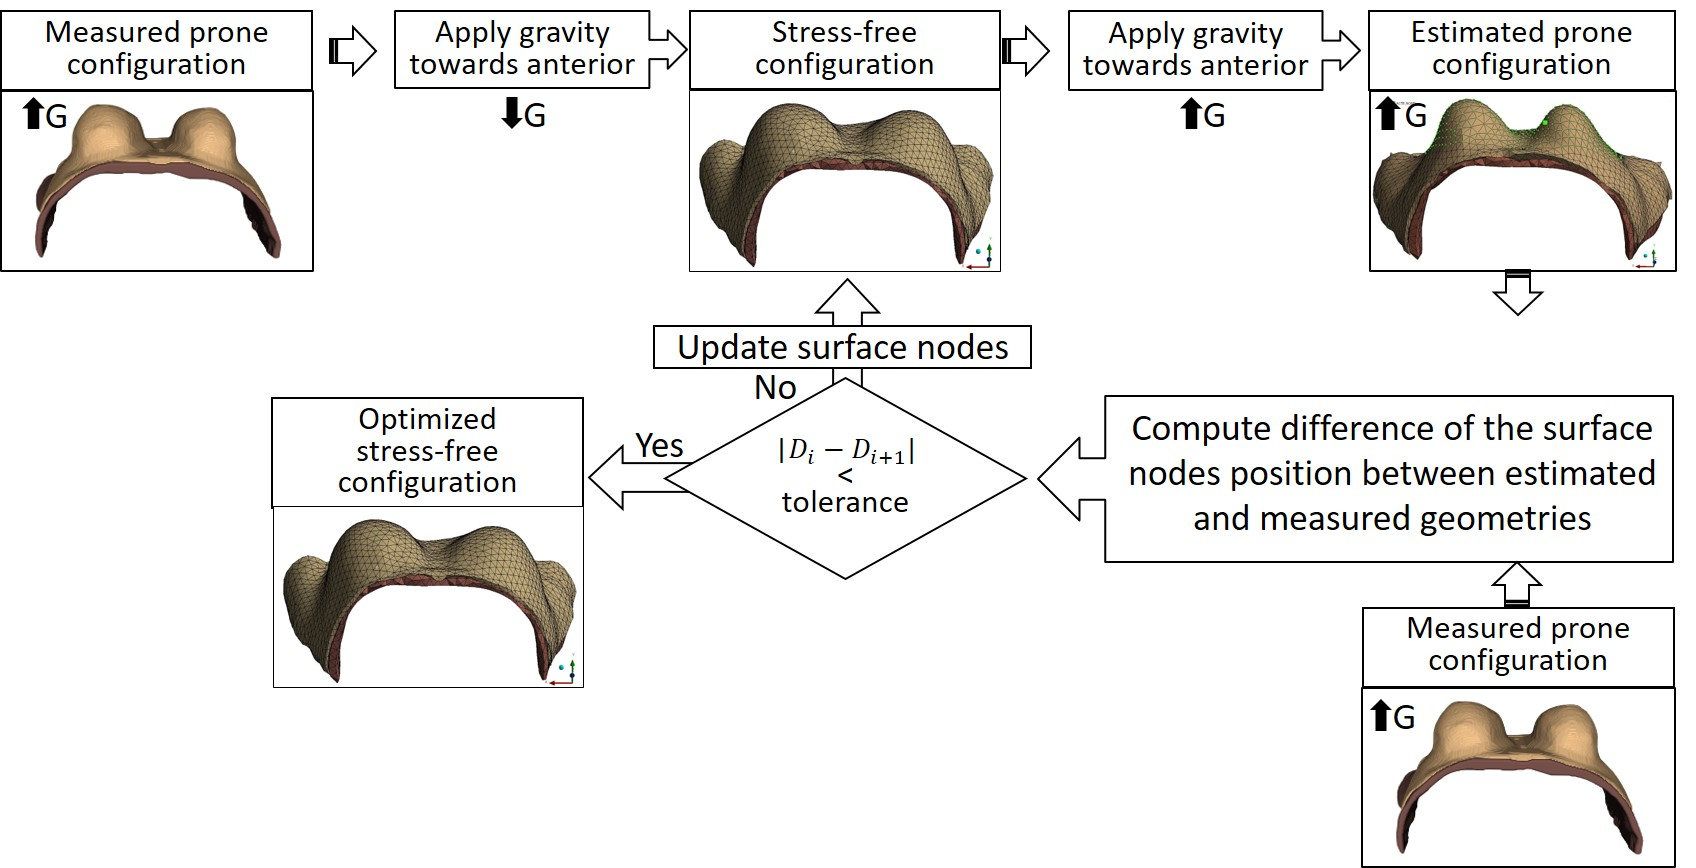
\includegraphics[width=1\textwidth,keepaspectratio]{figures/prediction-correction.jpg} 
\caption{Prediction-correction algorithm}\label{predictioncorectionalgo}
\end{figure}


 \subsubsection*{Inverse FE algorithm}
\cite{pathmanathan_predicting_2008} and later \cite{vavourakis_inverse_2016} proposed an analytic computation of the reference state of breast by reparametrizing the equilibrium equation and solving finite elements formulation of the inverse motion. The model provides good estimates of breast reference configurations but need large numerical resources. \cite{eiben_breast_2014} showed that, the prediction-correction iterative algorithm and the inverse FE algorithm are similar in terms of resulting accuracy. 

\readysubsection{Constitutive models}

Global breast mechanics are governed by breast tissue compositions and their individual mechanical properties. The breast soft tissues are known to be incompressibles, nonlinear, anisotropic, and viscous materials. However, according to \cite{wellman_breast_1999} the breast tissues viscosity can be neglected when the mechanical load is applied within short time scales.  

Under large compression and body position change the breast volume varies due to the blood flows, thus soft tissues are frequently modeled as quasi-incompressible materials with a Poisson ratio ranging between $\nu = {0.45-0.5}$. The influence of the Poisson ratio within linear constitutive models was studied by \cite{tanner_factors_2006}, according to the authors the best estimates are obtained with high Poisson ratio ($\nu = {0.495,0.499}$). The soft breast tissues are predominately composed of water; therefore, the density is considered to be equal to $9810 kg/m^3$.  


For the last decades several constitutive models were used to model the breast tissues response to a external force: exponential elastic \citep{azar_methods_2002}, Neo-Hookean hyper-elastic \citep{carter_biomechanical_2009,rajagopal_modeling_2010,sturgeon_finite_element_2016, eiben_breast_2016, han_nonlinear_2014, garcia_mapping_2017}, Money-Rivling \citep{samani_elastic_2007,tanner_factors_2006,carter_application_2012,martinez_finite_2017}. \cite{eder_comparison_2014} compared the most popular models in a multi-loading gravity simulation, according to the authors the Neo-Hookean model proposed by \cite{rajagopal_creating_2008} gives the best estimates.

\subsubsection*{Glandular and adipose tissues biomechanical properties }
 Multiple studies have shown that breast composition and so its mechanical behavior undergo substantial changes during woman lifetime (section \ref{subsection:adultbreasttexturechanges}). The first studies on mechanical proprieties estimation of breast tissues were done in diagnostic purposes. Then the breast is developing bening or malign disorders, their mechanical properties differ from the ones of the normal breast tissues.  In a study of 142 simples, bellowing to 4 type of tissues,  \cite{krouskop_elastic_1998} found that depending on the pre-compression level Young’s modulus of invasive carcinoma is from 5 to 25 times larger than the one of normal adipose tissue  ( from 5\% to 20\% pre-compression).  

Later, several research groups (Table \ref{table:materialproperties}) have studied the elastic modulus of adipose and glandular tissues. The breast tissues elastic parameters range between 0.1 kPa and 271.8 kPa. Such big variation may be explained by the differences in the used experimental set-up but also by the participant's physical condition, age or period of the menstrual cycle. For example, \cite{han_development_2012} though using the same FE method, found significantly inter-individual variability, with the shear modulus ranging between $0.22-43.64 kPa$. \cite{lorenzen_menstrual-cycle_2003} showed that during the menstrual cycle, due to the hormonal changes, the elastic properties of the glandular tissues can change by about 30\%.

\begin{table}[!h]
\centering
\begin{tabular}{|p{0.25\linewidth}|p{0.13\linewidth}|p{0.1\linewidth}|p{0.17\linewidth}|p{0.17\linewidth}|}
 \hline
\multicolumn{5}{|c|}{\textbf{Ex-vivo estimation}}\\ \hline

\multirow{2}{*}{ Author} & \multirow{2}{*}{ Method} &  Material & \multicolumn{2}{c|}{material properties}\\  \cline{4-5}

&& model &Adipose $kPa$ & Glandular $kPa$ \\  \hline

\cite{krouskop_elastic_1998} & Indentation-5\% . & Linear elastic & $E=19 \pm 7$ &$ E=33 \pm 11$ \\ \hline
 \cite{krouskop_elastic_1998}   & Indentation- 20\%& Linear elastic & $E=20 \pm 6  $& $E = 57 \pm 19 $ \\  \hline
 \cite{wellman_breast_1999}  & Indentation - 5\% & Linear elastic & $E=6.6 $ & $E= 33 $\\ \hline
 \cite{wellman_breast_1999}  & Indentation - 15\% & Linear elastic &$ E= 17.4 $& $E= 271.8 $ \\ \hline
 \cite{samani_method_2004} & Indentation & Linear elastic & $E = 3.25 \pm 0.91 $ & $E = 3.24 \pm 0.61 $ \\ \hline \hline
 \multicolumn{5}{|c|}{\textbf{In-vivo estimation}}\\ \hline
 \cite{van_initial_2003} & MRE & Linear elastic & $E = 17-26 $ & $E = 26-30 $ \\ \hline
 \cite{sinkus_viscoelastic_2005}&MRE& Visco-elastic & \multicolumn{2}{|c|}{$\mu = 2.9 \pm 0.3$} \\ \hline
 \cite{rajagopal_creating_2008}  & MRI-FEM& Neo-Hookean & $\mu = 0.16$ & $\mu = 0.26$ \\ \hline
 \cite{carter_determining_2009} & MRI-FEM& Neo-Hookean &$\mu = 0.25$ & $\mu = 0.4$ \\ \hline
 \cite{han_development_2012} & MRI-FEM & Neo-Hookean & $E= 1$ & $E = 0.22-43.64 $ \\ \hline 
 \cite{gamage_modelling_2012} & MRI-FEM & Neo-Hookean & \multicolumn{2}{|c|}{$\mu = 0.1 $} \\ \hline
 \cite{griesenauer_breast_2017} & MRI-FEM & Hooks law & $E = 0.25$ & $E = 2$\\ \hline
\end{tabular}
\caption{Material properties for adipose and glandular tissues.}
\label{table:materialproperties}
\end{table}

An important difference in estimated values of elastic modulus of breast soft tissues is observed between the linear elastic and hyperelastic models. If only in-vivo studies with Neo-Hookean material models are considered, the range of the adipose and glandular shear modulus is significantly lower than $ 50kPa$. 

\cite{carter_biomechanical_2009} compared one parameter Neo-Hookean potential function with five parameters Money-Rivling potential function for various material properties. The multy-loading gravity simulation were thus performed on 3 subjects. According to the authors the Money-Rivling models underestimates the tissues deformation by at least 75\% then the subject is re-positioned from the supine to the prone positions. The best estimates were given by the Neo-Hookean model with the initial shear modulus equal to $0.2kPa$.  

Previously listed researches clearly showed the variability of elastic modulus of the same tissue between and within individuals. \cite{eder_comparison_2014} made a larger analysis including all material models proposed in the literature. According to authors, many of them are too stiff permitting not enough deformation within the gravity loading. The most reliable identified values is the ones given by \cite{rajagopal_creating_2008} (Table \ref{table:materialproperties}).

\subsubsection*{Muscle biomechanical properties.} 
Muscle is a kinematically, geometrically, and materially complex tissue. Muscle mechanical behavior depends on its contractile active and passive elastic properties \citep{nordez_muscle_2010}. In biomechanics the muscle is modeled using complex models as Hill-type models
\citep{zajac_muscle_1989}, Feldman’s lambda model \citep{feldman_once_1986} which are considering the variation of muscle elasticity in function of muscle state. In breast biomechanical models the muscle is combined with the thoracic cage and is frequently considered as a rigid breast support. In most of models, the pectoral muscle is modeled by imposing zero-displacement conditions on nodes closer to the chest wall \citep{abbas_biomechanical_2001,chung_modelling_2008,rajagopal_mapping_2010}  
or by allowing them to slide along the chest wall line \citep{han_nonlinear_2014,georgii_simulation_2016}.   

The muscle is nonlinear, anisotropic, incompressible material.  The bibliographic data on static mechanical properties of the muscle-tendon unit assessed by supersonic shear wave imaging elastography state a Young's modullus in range of $20kPa$ to $300kPa$  depending on the muscle location and subject's physical condition \citep{lima_eassessment_2018}.  The muscle shear modulus on the upper trapezius was studied by \cite{leong_quantitative_2013}, according to authors the muscle shear elasticity  at rest was $17.11\pm 5.82 kPa$, and this increased to $26.56\pm 12.32 kPa$ during active arm holding at 30\textdegree  abduction. 

\subsubsection*{Skin biomechanical properties}
Several studies shown the importance of skin in biomechanical breast modeling. According to \cite{carter_biomechanical_2009}, a model which include the skin estimate better the tissues deformation under gravity loading.

 \cite{sutradhar_vivo_2013} published a complete study of breast skin estimating its elasticity for 16 different breast regions. The study was done on 23 female volunteers aging from 29 to 75 ears. The authors found that the skin elastic modulus range between $15-480 kPa$ with an average of $334\pm 88 kPa$. The elastic modulus in the lateral region (mean $370 kPa$) has the highest value followed by the superior region (mean $355 kPa$). The inferior region (mean $331 kPa$) follows next, with the medial region having the
lowest value (mean $316 kPa$). However, no significant variation of elastic modulus in radial direction was found. 
 
Other researches on skin elasticity are available, but they are not specific to the breast skin. \cite{hendriks_relative_2006} estimated in-vivo skin proprieties by suction testing. The skin was considered as a homogeneous, isotropic, incompressible, hyperelastic material. The study was performed on 14 subjects and the obtained average of elastic modulus for skin was $58.4 kPa$.

The estimation of the breast skin elasticity by the means of finite elements using Neo-Hookean potential function has resulted in softer materials model. \cite{carter_determining_2009} found a initial shear modulus equal to $16kPa$, whereas \cite{han_nonlinear_2014} found that for the five studied subjects the skin shear modulus ranged between $2.47 kPa$ and $5.78kPa$. 

\subsubsection*{Fascias and ligaments biomechanical properties}
The surrounding breast fascias and the supervisory ligament form the breast support matrix. These structures are wall described for surgical purposes (thickness, location etc), however little is known about their mechanical properties. The first biomechanical breast model taking into account the effect of Cooper's ligaments was proposed by \cite{azar_methods_2002} and took up later by \cite{pathmanathan_predicting_2008} and \cite{han_development_2012}. The authors designed a new material model for fatty tissues including the anisotropic behavior of breast ligaments. Later, \cite{georgii_simulation_2016} come up with a spring-mass generic model for the breast support matrix. According to the authors, including the ligaments into the finite elements breast model have increased the robustness of the prone-supine simulation with respect to the input parameters. 

 To our knowledge, where are no experimental data describing the mechanical properties of breast superficial fascia. An approximation of the elastic modulus of Cooper's ligaments is given by \cite{gefen_mechanics_2007} by extrapolating from known ligamentous structure in the human body. The authors estimated the elastic modulus of suspensory ligaments to relay between $80 - 400 MPa$
 
 %microscopic and macroscopic studi of fascia
 The fibrous tissues obtain their elasticity from elastic fibers and their structural support from collagen fibers. As reported by \cite{riggio_anatomical_2000} the superficial fascia is made up of both collagen and elastic fibers. In contrast, the Cooper's ligaments appeared to be composed almost of collagen fibers.  The mechanical properties of a single collagen fiber from a rat tail were studied by \cite{wenger_mechanical_2007}, according to authors their elastic modulus range between $5 GPa$ and $11 GPa$. Other studies on biomechanical characterization of human body superficial fascia are available in literature. The most frequently studied is on the plantar fascia and foot ligaments with a Young's modulus ranging between $0 MPa$ and $700 MPa$ \citep{cheung_effects_2004,kongsgaard_mechanical_2011}. 

\readysubsection{Boundary conditions}

Direclet conditions are usually used to constrain the sternum/axilla ends and the posterior surface of the breast or the thoracic cage if the muscular tissues are considered \citep{griesenauer_breast_2017,rajagopal_creating_2008,pathmanathan_predicting_2008, gamage_modelling_2012,griesenauer_breast_2017}. As reported by \cite{carter_biomechanical_2009} the zero-displacement boundary conditions in a multi-gravity loading framework result in a over-constrained model and sliding conditions on the mesh nodes corresponding to the chest wall have to be considered.    

  Later, several teams using biomechanical breast models for multy modality image registration or surgical planing showed what included the sliding boundary conditions  \citep{georgii_simulation_2016,han_nonlinear_2014}  improve the registration accuracy. However those studies were the biomechanical model is designed for breast compression, the tissues sliding over the chest wall is neglected and fixed boundary conditions are usually assumed \citep{sturgeon_finite_element_2016, martinez_finite_2017}.
  
 \readysubsection{Conclusion}
 
 During the last decades, several breast biomechanical models were proposed however, only a small part of them \citep{carter_biomechanical_2009,gamage_modelling_2012,han_nonlinear_2014} were evaluated with respect to the real tissues deformation. As we intend to build-up a subject specific breast biomechanical model capable of estimating multi-loading gravity deformations our assumption will rely only on already evaluated model within a same framework.
 
Today's outstanding breast biomechanical models are represented by the next three models:   \cite{eiben_surface_2016}, \cite{han_nonlinear_2014}, \cite{gamage_modelling_2012}.  \cite{gamage_modelling_2012} proposed a finite elements model capable to estimate the supine breast configuration from the prone one. To assess the quality of fit, the root-mean-squared error (RMSE) form the point to surface distance was computed.  Conform to the authors, the breast supine geometry was estimated within an RMSE of 5mm (maximal distance of 9.3 mm).  In the same time, \cite{han_nonlinear_2014} developed a breast biomechanical model for image registration. The estimates were computed for five subjects, and the accuracy was assessed by computing the Euclidian Distance (ED) between anatomical landmarks.  The mean ED range between 11.5 mm and 39.2 mm (maximal ED range between 20.3mm and 61.7mm).  Finally, \cite{eiben_surface_2016} proposed a new model to estimate the up-standing breast configuration from the prone one. The model was evaluated on 3 subject. The supine configuration was then computed from the prone one and the quality of fit was measured in terms of the mean Eulerian Distance between manually selected internal landmarks. Thus, the supine breast configuration was estimated within a mean distance ranging between $12.2mm$ and $19.8 mm$. The model evaluation for the up-standing configuration was not presented.   
 
 
\begin{sidewaystable}[!h]
    \centering
    \small
   \begin{tabularx}{22cm}{|p{2.5cm}|p{2.5cm}|p{3.5cm}|X|p{3.5cm}|p{2.5cm}|}
   \hline
   Authors & Application & FE mesh & Material models & Boundary conditions & Stress-free config. \\
\hline
  Azar F. et al. \citep{azar_methods_2002} &  Computer assisted breast surgery & 8-Node hexahedrons (trilinear isotropic elements) & Skin-elastic linear, 
   adipose,glamdular-hyperelastic polynomial & Sliding between breast - thorax and breast-paddle & Prone breast geometry\\
   \hline
 Rajagopal V. et al.  \citep{rajagopal_modelling_2007} & Breast compression & 8-Node hexahedrons (tricubic Hermite elements)& Homogeneous , Neo-Hookean model& Zero-displacement BC & Buoyant breast in water \\
   \hline
  Pathmanathan P. et al. \citep{pathmanathan_predicting_2008}&Image registration & 8-Node hexahedrons (trilinear elements)& Homogeneous breast-polynomial hyperelastic; Skin exponential hyperelastic  & Zero-displacement on muscle; Compression with imposed displacement & Inverse FE algorithm \\
   \hline
  Han L. et al. \citep{han_nonlinear_2014}& Image registration& 4-Node tetrahedrons & Muscle, glandular, fatty, skin - Neo-Hookean model & Sliding on pectoral muscle & Inverse gravity \\
   \hline
 Gamage T. et al.  \citep{gamage_modelling_2012}&  Computer assisted breast surgery & 8-Node hexahedrons (tricubic Hermite elements) & Homogeneous+ muscle- Neo-Hookean incompressible model& Zero-displacement BC on rib cage surface, Sternum, axilla ends, shoulder & PC iterative algorithm \\
   \hline
 Patete P. et al.  \cite{patete_multi_2013}& Computer assisted breast surgery& 4-Node tetrahedrons (trilinear isotropic elements) & Adipose , glandular, skin & Zero-displacement BC on the  chest wall&PC iterative algorithm\\
   \hline
 Kuhlmann M. et al. \citep{kuhlmann_mechanical_2013}& image registration & 4-Node tetrahedrons & Adipose, glandular- linear gel-like (Eulerian formulation); Skin - hyperelastic material (Lagrangian formulation) & Zero-displacement chest wall& PC iterative algorithm\\
   \hline
   
 Georgii J. et al.  \citep{georgii_simulation_2016}&Surgery simulation & 8-Node hexahedrons, 2-node 3D spars & homogeneous elastic material, Cooper's ligaments-generic mass-spring model & sliding BC (breast on the pectoral muscle) & NA\\
   \hline
  Eiben B. et al. \citep{eiben_surface_2016} & Surgery outcome prediction & 4-Node tetrahedrons & Fatty , glandular- Neo-Hookean model; skin- exponential hyperelastic & Zero-displacement BC & Inverse FE algorithm \\ 
   \hline
  Garcia E. et al. \citep{garcia_mapping_2017} & 3D breast lesion localization & 4-Node tetrahedrons & adipose, glandular  - Neo-Hookean models &zero-displacement BC & Prone breast configuration\\
   \hline
    \end{tabularx}
     \caption{Breast biomechanical models}
     \label{table:mechanical_models_table}
\end{sidewaystable}


%\end{table}
